\section{Challenges}
\label{sec:challenges}

As already stated above, nearly every web project bears challenges to solve, both for developers on the one hand, and for content creators on the other hand. While content creators mostly need to solve structural issues in the published content, developers are mainly responsible for supporting authors in technical questions, as well as constantly keeping an eye on the backend development. This might go from always keeping the underlying modules updated, to populating the source code with design or template changes, to finally maintaining the build pipeline and deployment setup.

\subsection{Distributed development}
\label{sec:challenges-distributeddevelopment}

When it comes to administer a static site project, it is very likely, that there will not be any possiblity of working on the same project in the same environment in a linear way. Instead, every developer will have to have a local install of the used generator at his/her disposal, together with access to a remote repository of a version control system for exchanging the current development status with other project maintainers. The main reason for that is the fact, that unlike content authors, developers do have the obligation of installing or maintaining the project's dependencies \cite[85]{dhillon2016}.

Content Editors on the other hand may, if using for example GitHub, make use of the remote "In-Page Code Editor" (see fig. \ref{fig:github-page-editor} on p. \pageref{fig:github-page-editor}), which also provides an optimistically rendered version of the current content, although without making use of the project's style sheet.

%% Graphic of separating project repositories
\begin{figure} % h-ere, t-op, b-ottom, p-age
    \centering
    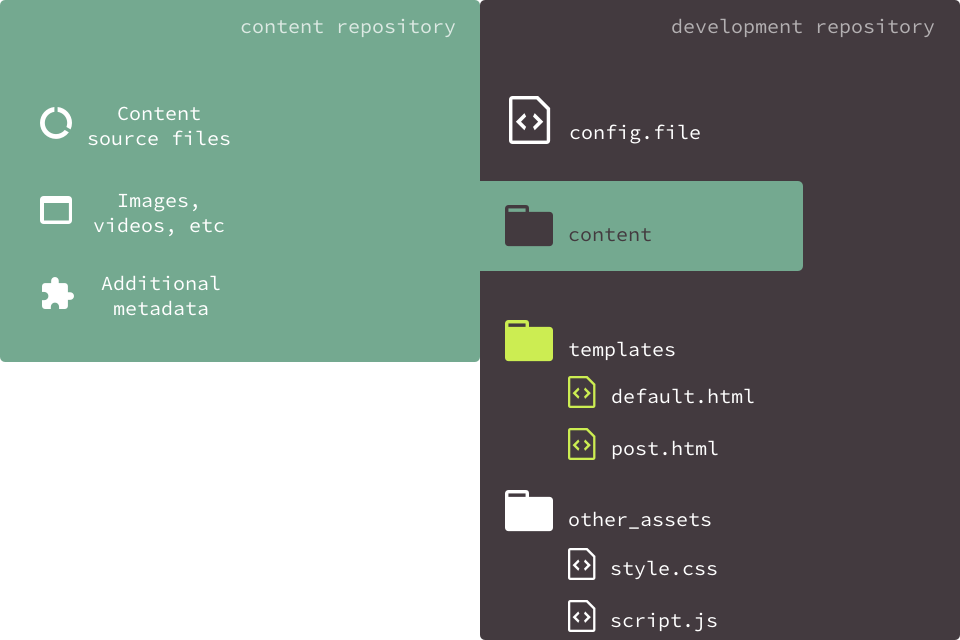
\includegraphics[width=0.9\textwidth]{challenges-repositories.png}
    \caption{A graphic showing the stylized separation of a project into a \emph{content} and a \emph{development} repository. The content authors may only be granted access to the content repository, while developers should be granted access to both, thus providing a seamless integration for the content into the build pipeline flow (see Fig. \ref{fig:build-pipeline} on p. \pageref{fig:build-pipeline}).}
    \label{fig:repository-separation}
\end{figure}
%

\subsubsection{Separating content from code}
As constantly growing static site projects may sooner or later come to a point, where content progression differs from development progression, it might be useful to separate both parts into independent repositories (see Fig. \ref{fig:repository-separation}). This especially makes sense, if the content editor team is also locally separated from the development team and therefore an additional level of security against accidental branch intermixture is needed.

\subsubsection{Merging only using pull requests}
However, if this kind of strong division is not desired anyhow, another option would be to limit access to the development repository in a way, that everyone may \emph{fork} a repository, but only certain project users are allowed to \emph{merge} external branches into the main development tree. On GitHub, \emph{pull requests} may be used. These pull requests allow any user to announce his/her contribution to the project using a commit history of a forked repository. The source project owners may then decide whether or not to merge the announced changes and also have the chance to express their point of view via comments directly on the pull request to its creator \cite[p. 394f]{loeliger2012version}.

The point in time, when a pull request is created is subsidiary, as further development on the specific branch is automatically included as well, as per-line comments are also removed, once the specific line of code has been modified in a following commit \cite{GithubPullRequests}. Furthermore, the possibility to merge is checked after every commit pushed to the respective branch, so the responsible users always know, if a merge operation may be successfully executed. Otherwise, a merge is only possible after locally checking out the pull request and processing it using the command line \cite{GithubMergePullRequests}.

\subsubsection{Staging versions}
Working with separate remote branches on a version control system like Git also allows for staging environments and therefore testing different versions of the projects concurrently. The public version however, visible to all clients visiting the website, remains stable and should receive only well-tested or well-considered updates as the very last step in the ongoing development.

To achieve this goal, a testbed is necessary and may be realized using another branch besides ``master''. Sometimes an additional ``bleeding edge'' version is also likely to be included in the build process. Based on this strategy, it is easy to control and maintain different revisions at the same time and nevertheless infer the functionality of different proof of concepts for merging them into the public version later on.


\subsection{Build cycles}
\label{sec:challenges-buildcyclecompletion}

One of the major challenges using static site generators remains the issue of providing a ``real website look and feel'' to the content editor. Whereas authors in dynamic CMSs are presented with an already pre-rendered version of the newly added content (since the underlying system is not dependent on any template rendering before deployment), static site generators only offer a glance of the author's work, after the whole build pipeline process succeeded in its render flow, unless other pre-caching methods are used. Yet, most static site generators do not include such kind of tools by default.

Based on the size and the amount of files in the website source code, this time frame can easily grow linearly. If there are also additional tasks added to the build process, such as resizing images to different screen sizes for providing a  responsive user experience, the computational effort may easily get out of hand and therefore the duration until the content editor first sees the result of his/her work simply gets unacceptable.

\subsubsection{Possible problems of long-lasting build processes}
Waiting for the completion of the build pipeline can cause severe recesses in the work performance of a content editor or developer, as further work depends on its success, while a failure is often combined with time loss beforehand and intensive bug hunting afterwards -- probably resulting in even more consecutive build pipeline failures. This assertion may not only be linked to crucial modifications in development, also the smallest hotfixes might as well provoke a full rebuild without justifying the whole effort.

Furthermore, being forced to wait in line may cause a developer to loose track on the development process, thus the introduction of hidden bugs (although not resulting in a build failure) is more likely. Additionally, mindlessly executing build cycles may even lead to data loss or blocking the workflow of other contributors.

%% Graphic of caching theory
\begin{figure} % h-ere, t-op, b-ottom, p-age
    \centering
    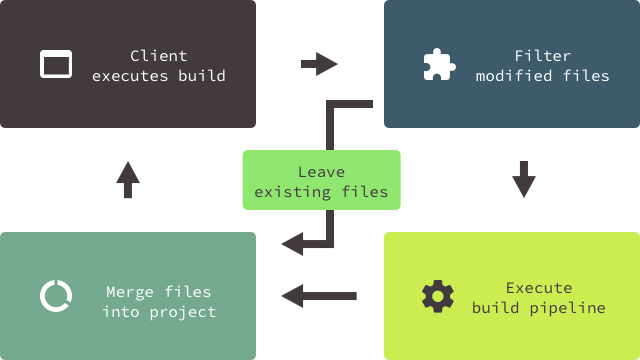
\includegraphics[width=0.9\textwidth]{challenges-caching.png}
    \caption{A graphic showing the theoretical approach of a build process flow, supported by caching.\\
    After the \emph{client} (content creator, developer) executes a build, the included caching mechanism should filter modified or added files and send them to the build pipeline. After the build succeeded, the newly built files should be merged with the already existing files to form an updated version of the website root.}
    \label{fig:caching}
\end{figure}
%

\subsection{Caching}
\label{sec:challenges-caching}
Speeding up a build process can be done via \emph{caching}. The right caching method should differ between unmodified content and files which actually have been reworked or were newly introduced into the project source. Using this sort of information, the algorithm might only choose the latter files, send them to the build pipeline and merge the outcome to the already existing project build (see Fig. \ref{fig:caching}).

Although a few static site generators already include some sort of caching methods -- although most of them only work locally (like Hexo's Warehouse, see ch. \ref{sec:hexo-technology}), a first step is made. It should significantly improve the build duration for local development, as long as the optimal cache storage is being used. Hexo's Warehouse uses a JSON file as persistant storage, while the temporary storage lies in the Computer's RAM. This is fine for smaller projects, but could also lead to critical memory issues when used in projects containing a huge amount of files. For bigger data sets, it would be possible to use caching in conjunction with databases like SQLite using the \emph{JSON1}\footnote{\url{https://www.sqlite.org/json1.html} -- JSON1 documentation on SQLite's website.} extension.

As the local cache may not easily be transferred to other contributors or deployment engines, the first build after a pull does not take advantage of any speed up technique. Moreover, the methods mentioned above all use a significant amount of local computing power to provide a useable cache, which could lead to problems and unwanted slowdowns on portable devices.

\subsubsection{Determination of cacheable contents}
\label{sec:challenges-cachedetermination}
The next step would be to select cacheable files, as not every file has the same impact on the project source. While normal blog posts are mostly self-contained --  unless there is probably a preview of a post featured somewhere, a template file on the other hand, is often a dependency for many blog posts. A working cache is more important for a commit only containing blog posts, than for a commit which only contains template files, as a template file acts as a dependency for possibly multiple content files. Therefore a template file invalidates the cache, which leads to a complete rebuild.

Since the relations between files, as well as their dependencies, may appear a bit obscure at first sight, it needs some kind of tracking system for ensuring a persistent overview of cacheable contents. This does not stop at comparing the file path within the project tree, as for example, all template files are stored within one special directory. For future considerations, also the source code would have to be examined, as the frontmatter in content files may contain information about dependencies to external files (see ch. \ref{sec:buildpipelines-frontmatter} on p. \pageref{sec:buildpipelines-frontmatter}). Therefore, the challenge here would be a reverse lookup mechanism for spotting file relations in the project source.
